\section{Appendix}\label{sec:Appendix}


\begin{figure}[!h]
    \centering
    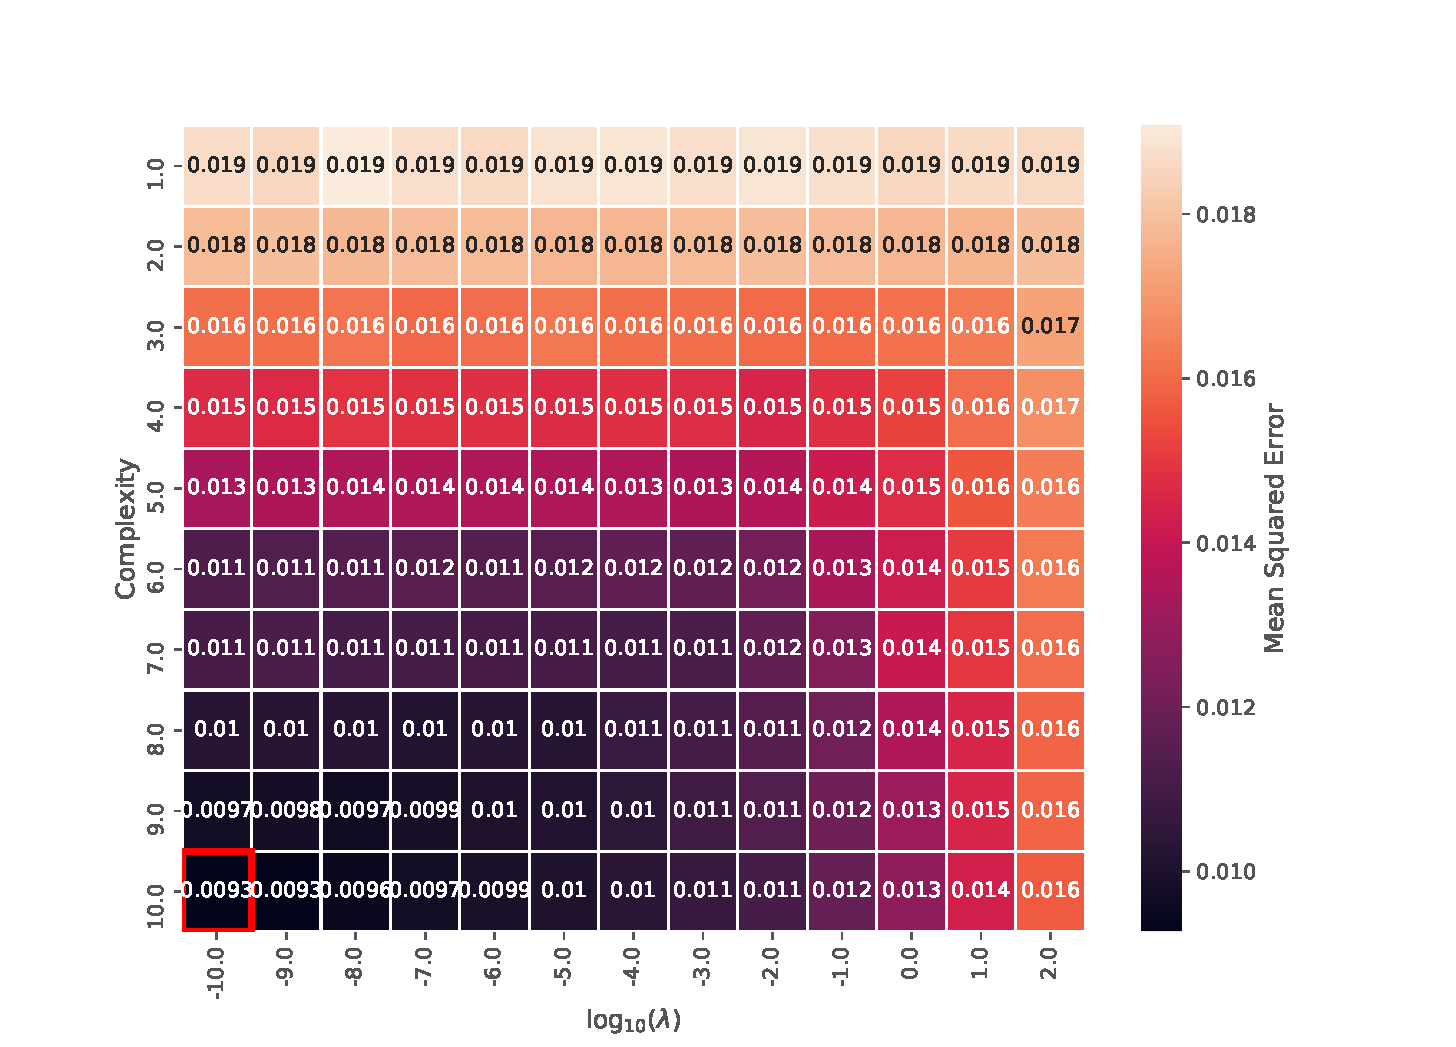
\includegraphics[scale=0.45]{Figures/APPENDIX/min_mse_heatmap_ridge_010.pdf}
    \caption{Heat map of the estimated MSE of Ridge method on the terrain data for value ranges of $\lambda$ and model complexity $d$.}
    \label{fig:appendix_heatmap_ridge}
\end{figure}

\begin{figure}[!h]
    \centering
    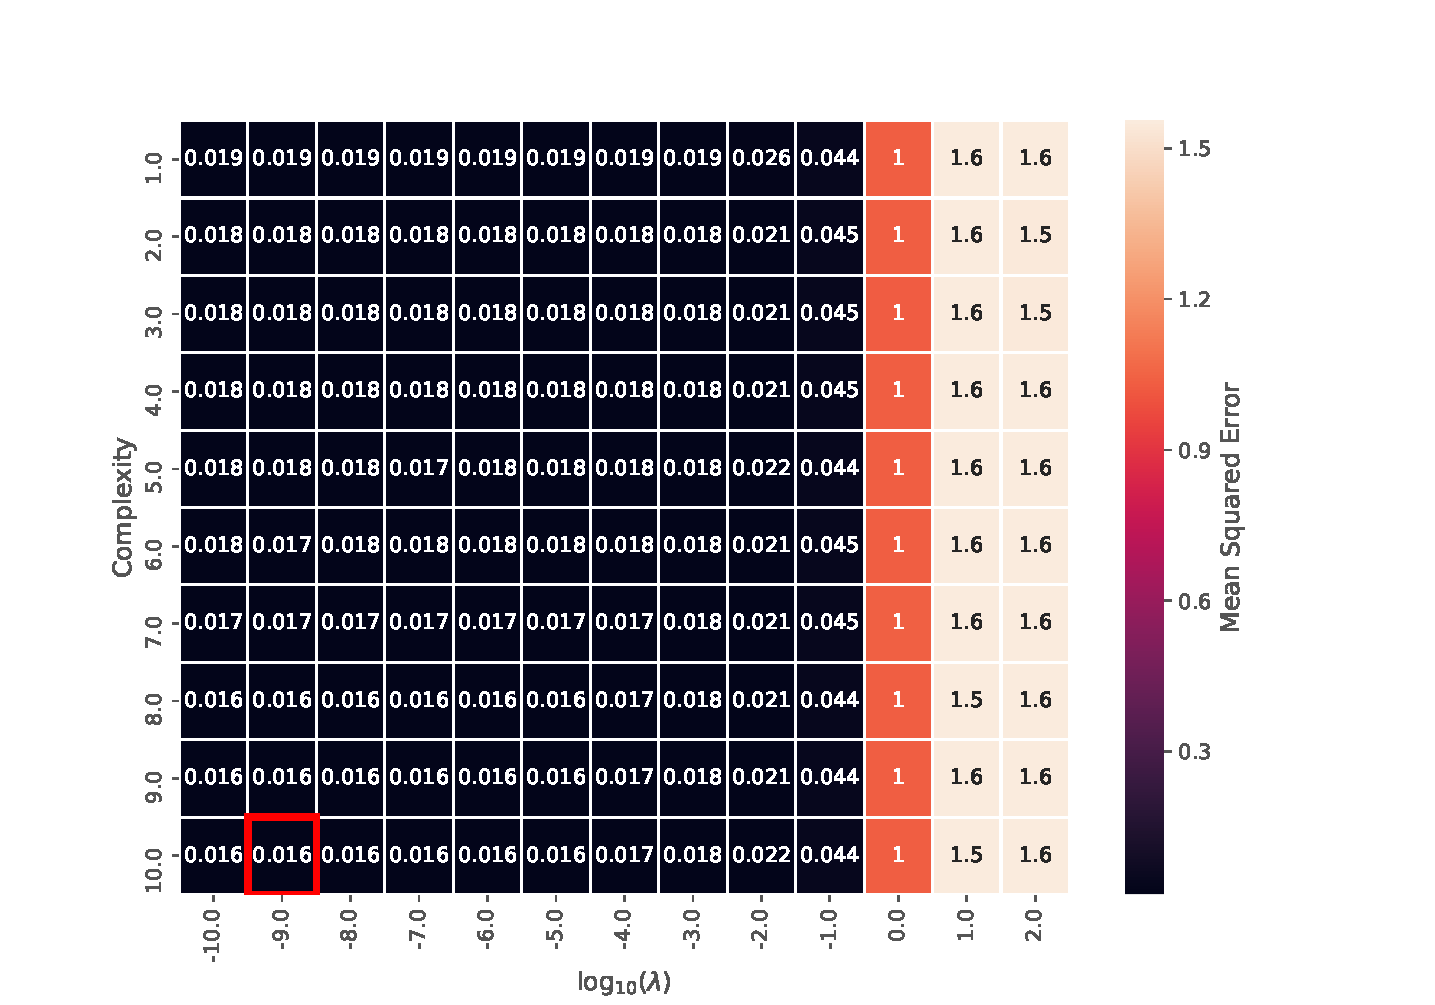
\includegraphics[scale=0.45]{Figures/APPENDIX/min_mse_heatmap_lasso_027.pdf}
    \caption{Heat map of the estimated MSE of the Lasso method on the terrain data for value ranges of $\lambda$ and model complexity $d$.}
    \label{fig:appendix_heatmap_lasso}
\end{figure}

\begin{figure}[!h]
    \centering
    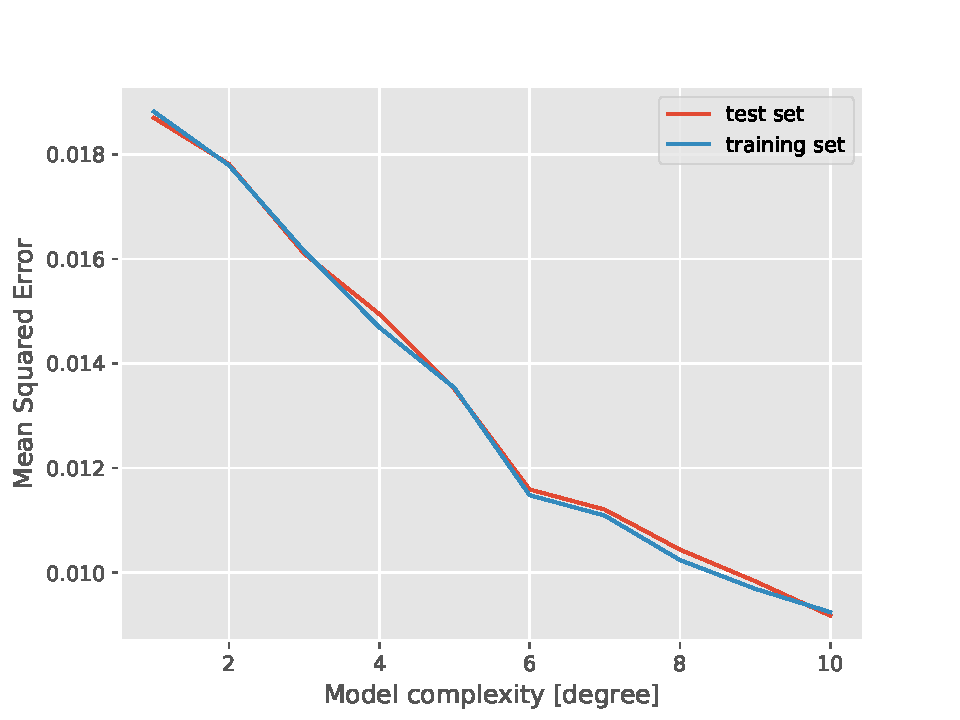
\includegraphics[scale=0.48]{Figures/APPENDIX/deg_analysis_ols_test_train_015.pdf}
    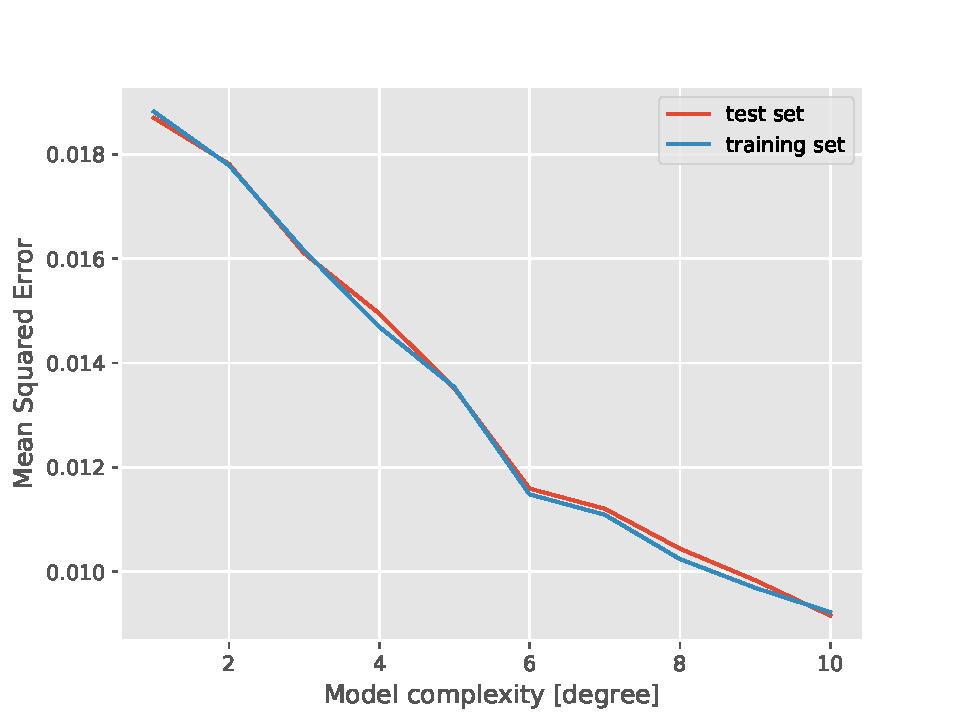
\includegraphics[scale=0.48]{Figures/APPENDIX/deg_analysis_ridge_test_train_011.pdf}
    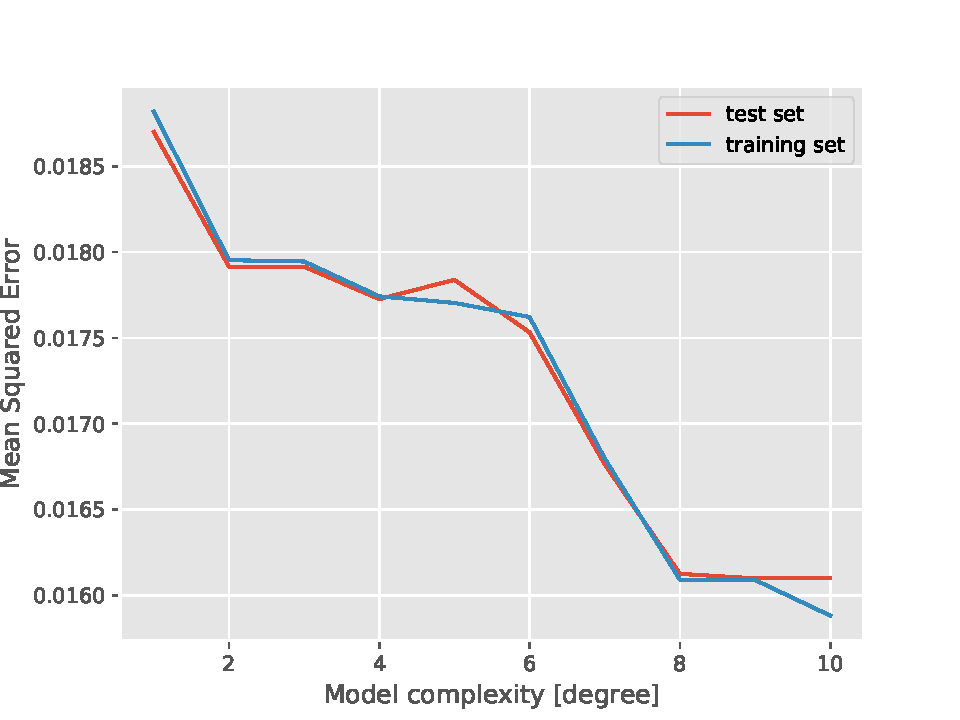
\includegraphics[scale=0.48]{Figures/APPENDIX/deg_analysis_lasso_test_train_025.pdf}
    \caption{MSE of the predictions by the OLS(top left), Ridge(top right) and Lasso(bottom) methods on the training and testing portions of the terrain data for different model complexities. $\lambda_{Ridge} = 10^{-10}$, $\lambda_{Lasso} = 10^{-9}$.}
    \label{fig:appendix_train_test}
\end{figure}

